%%%%%%%%%%%%%%%%%%%%%%%%%%%%%%%%%%%%%%%%%%%%%%%%%%%%%%%%%%%%%%%%%%%%%%
% Template para artigos da SBC
% Adaptado para o trabalho prático de Processamento de Dados com Grafos
%%%%%%%%%%%%%%%%%%%%%%%%%%%%%%%%%%%%%%%%%%%%%%%%%%%%%%%%%%%%%%%%%%%%%%

\documentclass[12pt]{article}

\usepackage{sbc-template}
\usepackage{graphicx,url}
\usepackage[utf8]{inputenc}
\usepackage{amsmath} % Para ambientes matemáticos
\usepackage{listings} % Para blocos de código
\usepackage{xcolor} % Para cores no código
\usepackage{placeins}

% Configuração para blocos de código
\definecolor{codegreen}{rgb}{0,0.6,0}
\definecolor{codegray}{rgb}{0.5,0.5,0.5}
\definecolor{codepurple}{rgb}{0.58,0,0.82}
\definecolor{backcolour}{rgb}{0.95,0.95,0.92}

\lstdefinestyle{customStyle}{
    backgroundcolor=\color{backcolour},
    commentstyle=\color{codegreen},
    keywordstyle=\color{magenta},
    numberstyle=\tiny\color{codegray},
    stringstyle=\color{codepurple},
    basicstyle=\ttfamily\footnotesize,
    breakatwhitespace=false,
    breaklines=true,
    captionpos=b,
    keepspaces=true,
    numbers=left,
    numbersep=5pt,
    showspaces=false,
    showstringspaces=false,
    showtabs=false,
    tabsize=2
}
\lstset{style=customStyle}

\sloppy

\title{Gestão de Dependências em Projetos Go com Ordenação Topológica}

% TODO: PREENCHER OS DADOS DOS AUTORES E INSTITUIÇÕES
\author{Nicholas Pereira Cristófaro\inst{1}, Nome Sobrenome do Aluno 2\inst{1}}

\address{Pontifícia Universidade Católica de Minas Gerais\\
  Belo Horizonte -- Minas Gerais -- Brasil
  \email{nicholaspcr@gmail.com, email2@dominio.com}
}

\begin{document}

\maketitle

\begin{resumo}
A gestão de dependências é um desafio em software moderno. Este artigo apresenta uma ferramenta que analisa e visualiza dependências em projetos Go, modelando-as como um grafo direcionado. Através da ordenação topológica com o algoritmo de Kahn, a ferramenta determina a sequência de compilação segura e detecta dependências cíclicas — um erro crítico em Go. A solução, implementada em Python, abrange desde a análise do código até a geração de um grafo interativo, oferecendo um suporte prático para a gestão de conflitos em sistemas de dependência.
\end{resumo}

\begin{abstract}
Dependency management is a challenge in modern software. This paper introduces a tool that analyzes and visualizes dependencies in Go projects by modeling them as a directed graph. Through topological sorting with Kahn's algorithm, the tool determines a safe compilation sequence and detects cyclic dependencies—a critical error in Go. The solution, implemented in Python, covers the process from code analysis to generating an interactive graph, providing practical support for managing conflicts in dependency systems.
\end{abstract}

\section{Introdução}

O desenvolvimento de software contemporâneo é caracterizado pela modularidade e reutilização de código, resultando em sistemas compostos por um grande número de componentes interdependentes. A gestão dessa rede de dependências é um desafio central na engenharia de software, por vezes referido como "inferno de dependências" \cite{jergensen2011}. Falhas nesse gerenciamento podem levar a erros de compilação, comportamento inesperado e dificuldades na manutenção.

A linguagem de programação Go (Golang) possui um sistema de pacotes estático e um compilador que impõem regras estritas sobre as dependências. Uma dessas regras é que as dependências de um pacote devem ser inicializadas antes do próprio pacote \cite{donovan2015go}. Isso garante a execução correta das funções \texttt{init()}, que configuram o estado inicial de cada pacote. Quando um projeto contém uma dependência cíclica, o compilador Go gera um erro, pois não é possível determinar uma ordem de inicialização válida \cite{GoSpec}.

A ordem de inicialização de pacotes em Go pode ser modelada como um grafo de dependências direcionado acíclico (DAG). A solução para determinar a sequência correta é, portanto, encontrar uma ordenação topológica desse grafo \cite{clrs}. Este trabalho detalha uma ferramenta que aplica esses conceitos para analisar projetos Go. Este trabalho se enquadra na proposta de "Gestão de Conflitos em Sistemas de Dependência", focando na modelagem, detecção de ciclos e execução segura baseada em ordenação topológica. Para isso, foi desenvolvida uma ferramenta em Python que analisa os arquivos, constrói o grafo de dependências, aplica o algoritmo de Kahn e gera uma visualização gráfica do resultado.

O restante deste artigo está organizado da seguinte forma: a Seção 2 apresenta a fundamentação teórica. A Seção 3 detalha a modelagem e a arquitetura da ferramenta. A Seção 4 apresenta estudos de caso e discute os resultados. Finalmente, a Seção 5 conclui o trabalho.

\section{Fundamentação Teórica}
Esta seção aborda os conceitos fundamentais que sustentam o desenvolvimento deste trabalho.

\subsection{Teoria dos Grafos}
Um grafo $G = (V, E)$ é uma estrutura matemática usada para modelar relações entre objetos, consistindo em um conjunto de vértices $V$ e um conjunto de arestas $E$ que conectam pares de vértices \cite{clrs}. Em um \textbf{grafo direcionado} (ou digrafo), as arestas são pares ordenados de vértices $(u, v)$, indicando uma ligação de $u$ para $v$. Um \textbf{caminho} em um digrafo é uma sequência de vértices onde cada vértice consecutivo na sequência está conectado por uma aresta direcionada. Um \textbf{ciclo} é um caminho que começa e termina no mesmo vértice.

Um \textbf{Grafo Acíclico Direcionado (DAG)} é um grafo direcionado que não contém ciclos. Esta estrutura é fundamental
para modelar problemas de pré-requisitos, como as dependências de software, onde um ciclo representaria uma condição ilógica (e.g., A depende de B, e B depende de A).

\subsection{Ordenação Topológica}
A ordenação topológica de um DAG é uma ordenação linear de seus vértices tal que para toda aresta direcionada $(u, v)$, o vértice $u$ vem antes de $v$ na ordenação \cite{clrs}. Se o grafo contiver um ciclo, não há ordenação topológica possível, o que, no nosso contexto, corresponde a um erro de "dependência cíclica". A Figura~\ref{fig:grafo-ciclico} ilustra um exemplo de um grafo com dependências cíclicas, onde é impossível determinar uma ordem de precedência linear entre os nós.

\begin{figure}[htbp]
    \centering
    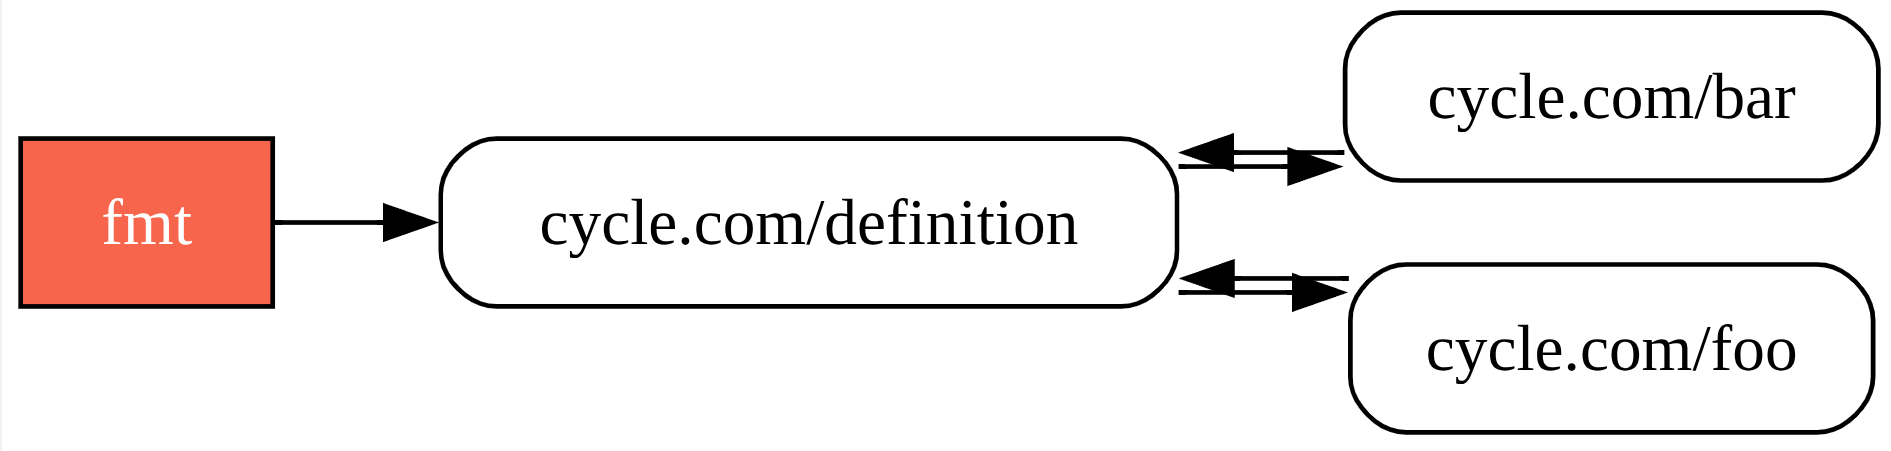
\includegraphics[width=1\textwidth]{examples/cycle.png}
    \caption{Exemplo de um grafo com uma dependência cíclica. O pacote `definition` depende de `foo` e `bar`, que, por sua vez, dependem de `definition`. Essa estrutura impede a criação de uma ordenação topológica.}
    \label{fig:grafo-ciclico}
\end{figure}

\FloatBarrier

Existem duas abordagens principais para a ordenação topológica:

\begin{itemize}
    \item \textbf{Baseada em Busca em Profundidade (DFS):} Este algoritmo realiza uma busca em profundidade no grafo. A ordenação topológica é a ordem inversa da finalização dos vértices. É eficiente, mas menos intuitivo para visualizar camadas de dependência.
    \item \textbf{Algoritmo de Kahn:} Baseado na remoção sucessiva de vértices sem dependências de entrada. Foi o escolhido para este trabalho por sua capacidade de agrupar os nós em "camadas", o que é ideal para a visualização proposta.
\end{itemize}

\subsubsection{Algoritmo de Kahn}
O algoritmo de Kahn, proposto em 1962, é uma abordagem clássica para a ordenação topológica \cite{kahn1962}. Ele funciona de maneira iterativa, processando vértices que não possuem mais dependências não resolvidas. O algoritmo baseia-se no cálculo do grau de entrada (\textit{in-degree}) de cada vértice e utiliza uma fila para armazenar os vértices com grau de entrada zero. A Listagem \ref{lst:kahn-pseudocode} apresenta o pseudocódigo do algoritmo.

\begin{lstlisting}[language={}, caption={Pseudocódigo do Algoritmo de Kahn}, label={lst:kahn-pseudocode}]
L = Lista vazia que contera os elementos ordenados
S = Conjunto de todos os nos sem arestas de entrada (in-degree 0)

enquanto S nao esta vazio faca
  remover um no n de S
  adicionar n em L

  para cada no m com uma aresta e de n para m faca
    remover aresta e do grafo
    se m nao tem mais arestas de entrada entao
      inserir m em S

se o grafo ainda contem arestas entao
  retornar erro (grafo tem pelo menos um ciclo)
senao
  retornar L (a ordenacao topologica)
\end{lstlisting}

Se, ao final, a lista `L` contém todos os vértices do grafo, a ordenação foi bem-sucedida. Caso contrário, o grafo possui um ciclo, e o algoritmo falha em processar todos os nós \cite{kahn1962}.

\subsection{Sistema de Pacotes e Módulos em Go}
Go organiza o código em pacotes, e a diretiva \texttt{import} é usada para declarar dependências \cite{donovan2015go}. A especificação da linguagem determina que a ordem de inicialização dos pacotes siga a ordem de dependência, um processo que é, na prática, uma ordenação topológica. A função \texttt{init} de um pacote é executada somente após todas as suas dependências terem sido inicializadas \cite{GoSpec}. O arquivo `go.mod` na raiz do projeto define o módulo e suas dependências diretas, sendo crucial para a resolução de pacotes.

\section{Modelagem e Desenvolvimento da Ferramenta}
Esta seção descreve a arquitetura e os componentes da ferramenta desenvolvida, detalhando como o problema de análise de dependências foi modelado e implementado em Python.

\subsection{Modelagem do Grafo de Dependências}
O problema foi modelado como um grafo direcionado $G = (V, E)$, onde $V$ é o conjunto de pacotes Go e uma aresta $(u, v)$ significa que o pacote $v$ importa o pacote $u$ (ou seja, $v$ depende de $u$). Essa direção é fundamental para que a ordenação topológica resulte em uma lista onde as dependências vêm antes dos dependentes. A estrutura de dados escolhida foi um dicionário (hash map) em Python, por sua eficiência em tempo de acesso.

\subsection{Componentes da Ferramenta}
A arquitetura geral da ferramenta, que segue o fluxo de extração, processamento e visualização, está ilustrada no diagrama de componentes da Figura~\ref{fig:diagrama-classes}.

\begin{figure}[htbp]
    \centering
    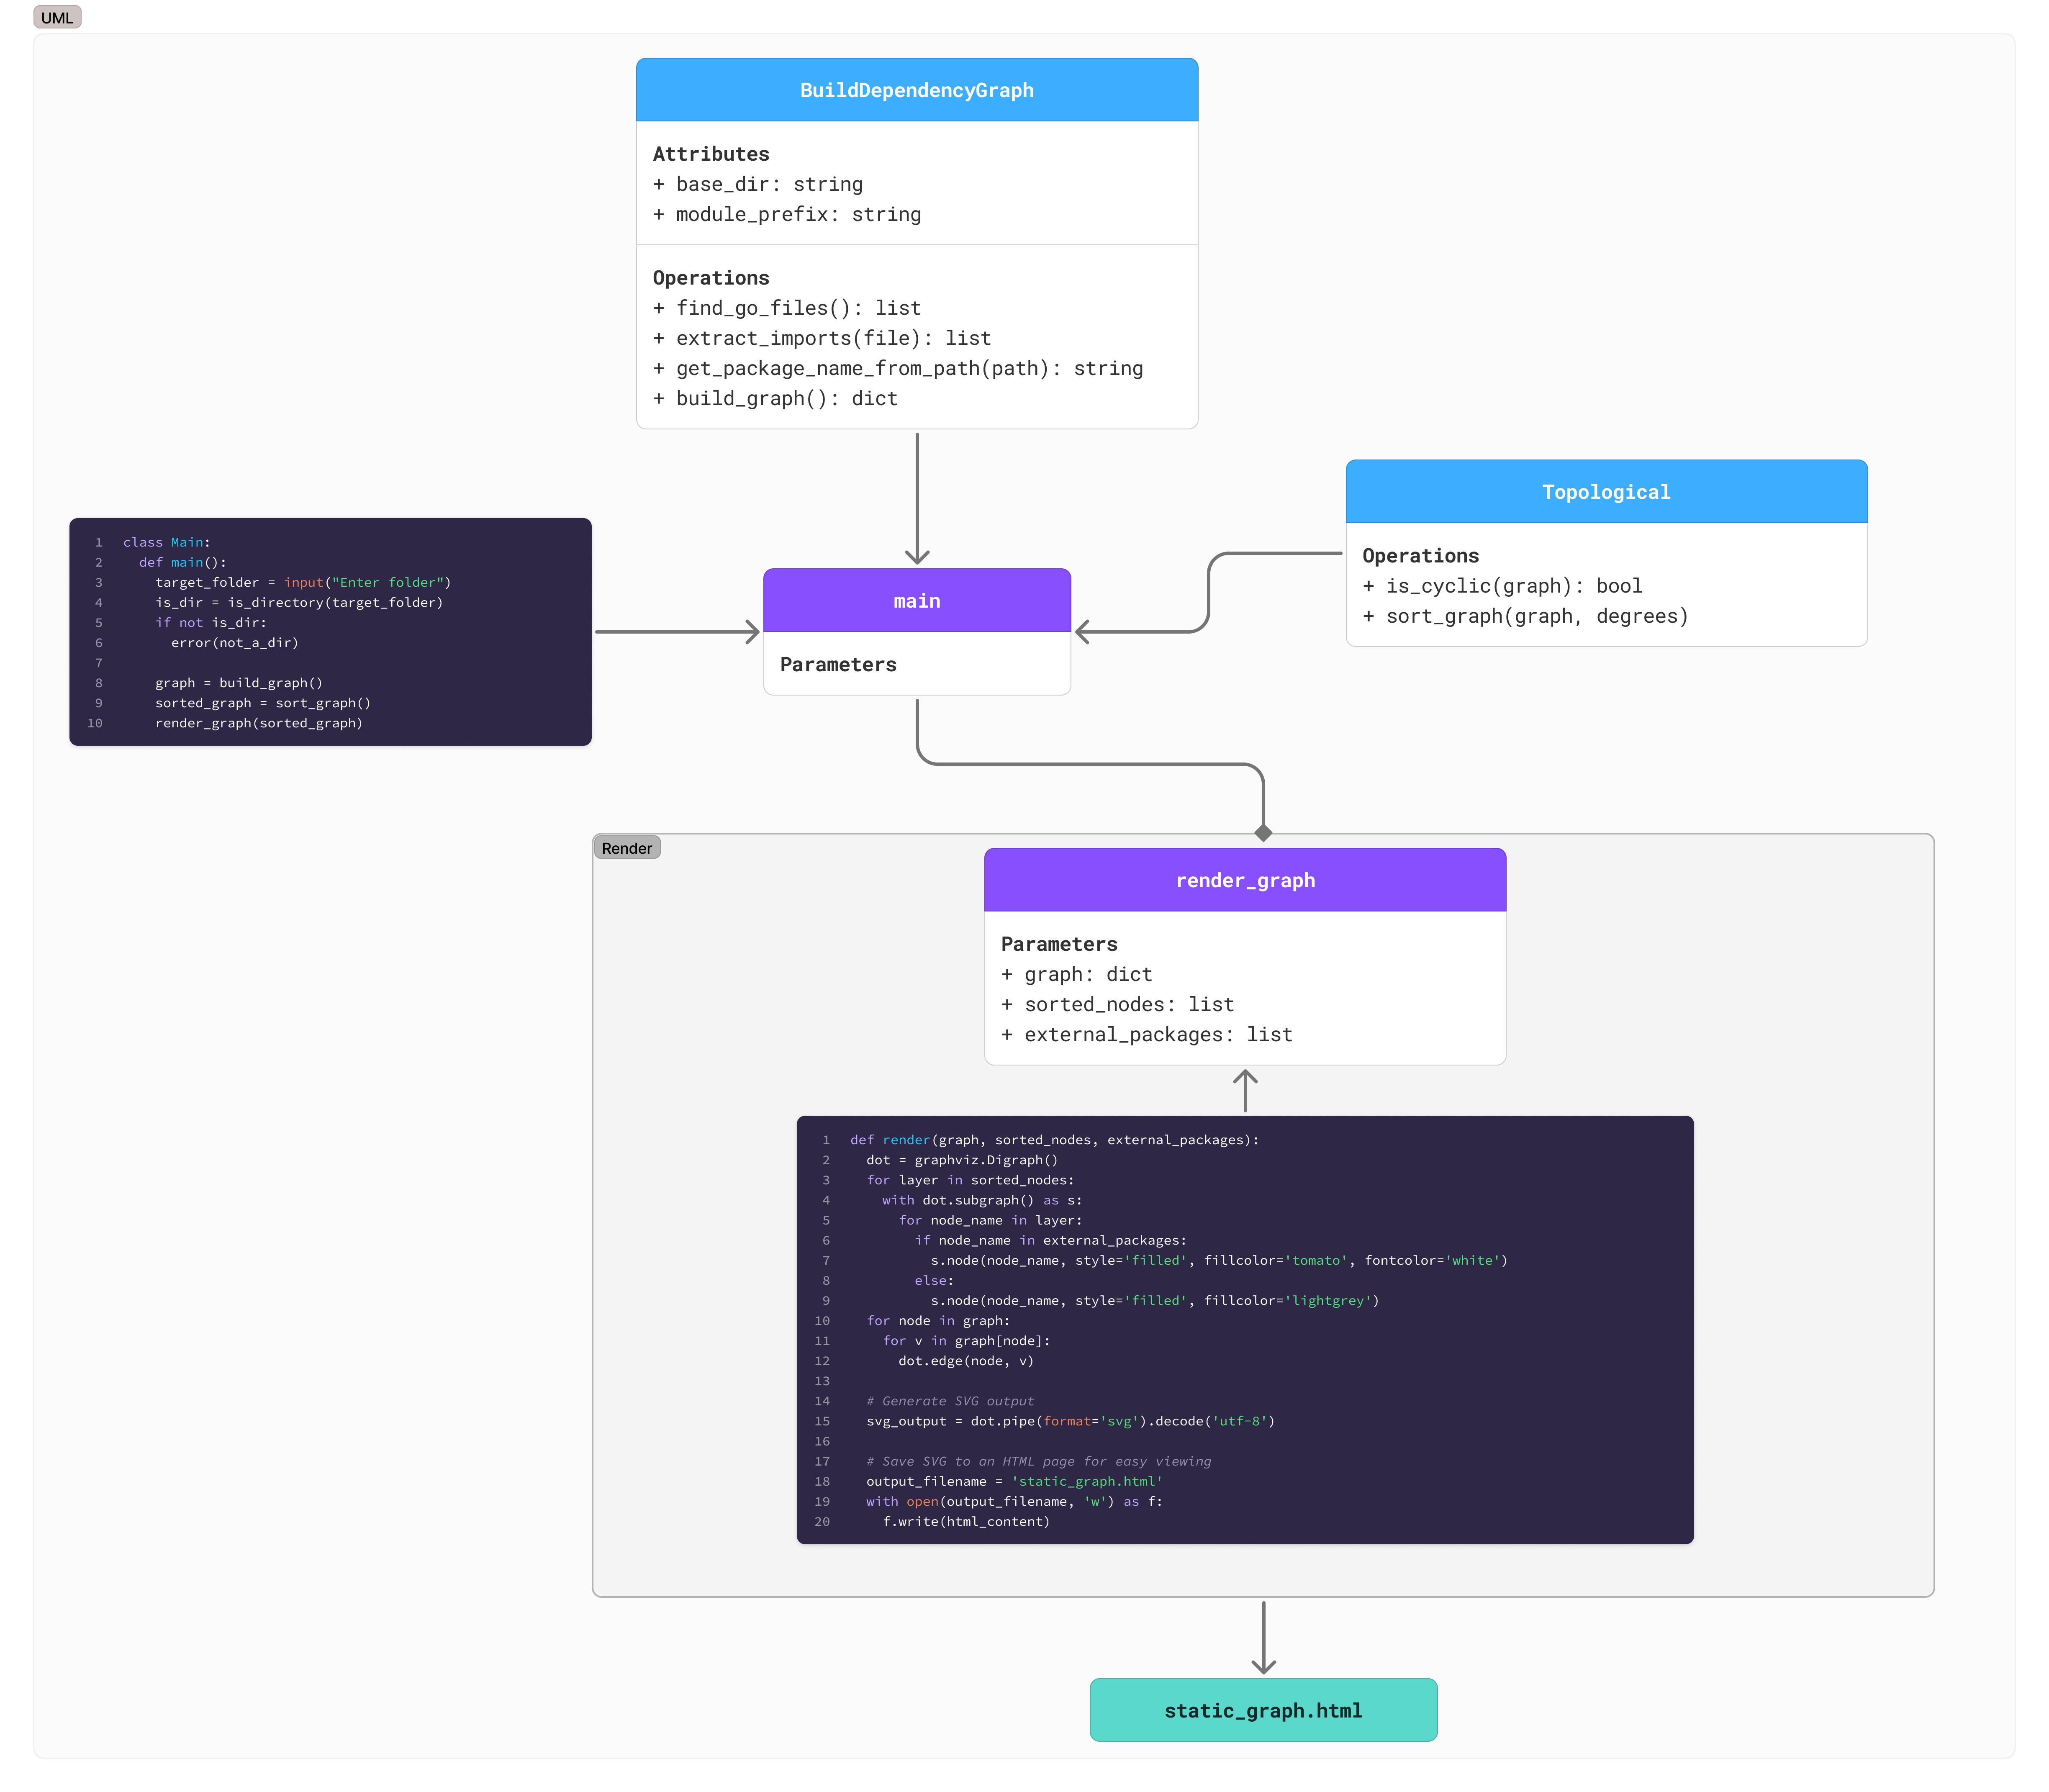
\includegraphics[width=0.75\textwidth]{images/diagrama_classes.png}
    \caption{Diagrama de componentes da ferramenta, ilustrando a interação entre os módulos de extração (\texttt{BuildDependencyGraph}), processamento (\texttt{Topological}) e renderização (\texttt{render\_graph}).}
    \label{fig:diagrama-classes}
\end{figure}

\FloatBarrier


A ferramenta é composta por três módulos principais, conforme os arquivos \texttt{dependency\_graph\_builder.py}, \texttt{topological\_sorting.py} e \texttt{render.py}.

\subsubsection{Extração e Construção do Grafo}
A extração de dependências é o primeiro passo e é implementada no módulo \texttt{dependency\_graph\_builder.py}. A lógica central está na função \texttt{extract\_imports}, mostrada na Listagem~\ref{lst:extract-imports}, que utiliza expressões regulares para analisar o conteúdo de cada arquivo Go.

\begin{lstlisting}[language=Python, caption={Trecho do código de extração de importações.}, label={lst:extract-imports}]
@staticmethod
def extract_imports(file_path):
    imports = set()
    with open(file_path, 'r', encoding='utf-8') as f:
        content = f.read()

    # Encontra blocos de importacao: import (...)
    import_block_match = re.search(r'import\s+\((.*?)\)', content, re.DOTALL)
    if import_block_match:
        block_content = import_block_match.group(1)
        found_imports = re.findall(r'"([^"]+)"', block_content)
        for imp in found_imports:
            imports.add(imp)

    # Encontra importacoes de linha unica: import "..."
    single_imports = re.findall(r'import\s+"([^"]+)"', content)
    for imp in single_imports:
        imports.add(imp)

    return imports
\end{lstlisting}

Esta abordagem com duas expressões regulares distintas garante que tanto importações de linha única quanto blocos de importação sejam corretamente identificados. Embora eficaz, o uso de regex pode ser frágil a formatações de código muito atípicas.

\subsubsection{Ordenação Topológica e Detecção de Ciclos}
Após a construção do grafo, o módulo \texttt{topological\_sorting.py} implementa a lógica de ordenação. Primeiramente,
um método de busca em profundidade, `is{\_}cyclic`, é invocado para garantir que o grafo é um DAG. Em seguida, o método
`sort{\_}group`, mostrado na Listagem \ref{lst:sort-group}, executa o algoritmo de Kahn.

\begin{lstlisting}[language=Python, caption={Trecho do código de ordenação topológica (Kahn).}, label={lst:sort-group}]
def sort_group(self, graph: defaultdict[str, set], in_degree: defaultdict[str, int]) -> list[str]:
    queue = deque()
    leaves_matrix: list[str] = []

    leaves_nodes = []
    for v in graph:
        if in_degree[v] == 0:
            leaves_nodes.append(v)
    queue.append(leaves_nodes)

    while queue:
        leaves_list = queue.popleft()
        leaves_matrix.append(leaves_list)
        new_leaves = []

        for node in leaves_list:
            for v in graph[node]:
                in_degree[v] -= 1
                if in_degree[v] == 0:
                    new_leaves.append(v)

        if new_leaves:
            queue.append(new_leaves)

    return leaves_matrix
\end{lstlisting}

A implementação utiliza uma `deque` da biblioteca `collections` para uma performance eficiente de enfileirar e desenfileirar. A principal característica desta implementação é o processamento em "camadas", que agrupa todos os nós que podem ser processados, formando a base para a visualização hierárquica.

\subsubsection{Visualização dos Resultados}
Finalmente, o módulo \texttt{render.py} é responsável por traduzir a estrutura de dados do grafo em uma imagem. A biblioteca `graphviz` \cite{graphviz} foi escolhida para esta tarefa. O trecho de código mais relevante é aquele que agrupa os nós em subgrafos com o mesmo `rank`, como mostra a Listagem \ref{lst:render}.

\begin{lstlisting}[language=Python, caption={Trecho do código de renderização do grafo.}, label={lst:render}]
def render(graph, sorted_nodes, external_packages):
    dot = graphviz.Digraph('DependencyGraph')
    dot.attr(rankdir='LR') # Layout da esquerda para a direita

    # Agrupa nos em subgrafos para alinhamento em camadas
    for layer in sorted_nodes:
        with dot.subgraph() as s:
            s.attr(rank='same') # Forca o mesmo rank (alinhamento)
            for node_name in layer:
                # Colore nos externos de forma diferente
                if node_name in external_packages:
                    s.node(node_name, style='filled', fillcolor='tomato')
                else:
                    s.node(node_name, style='filled', fillcolor='lightgrey')

    # Adiciona as arestas ao grafo
    for node in graph:
        for v in graph[node]:
            dot.edge(node, v)

    # Gera o arquivo final (SVG embutido em HTML)
    ...
\end{lstlisting}

A diretiva `rank='same'` é o que garante que todos os pacotes em uma mesma camada da ordenação topológica sejam alinhados verticalmente, tornando a hierarquia de dependências clara e intuitiva.

\section{Aplicação e Resultados}
Para validar a ferramenta e demonstrar sua utilidade, ela foi aplicada a projetos com diferentes níveis de complexidade. Esta seção apresenta uma análise dos grafos gerados.

\subsection{Estudo de Caso com Projetos Reais}

\subsubsection{Caso 1: Aplicação Simples}
O primeiro cenário, ilustrado na Figura \ref{fig:grafoExemplo}, representa uma aplicação web hipotética. O grafo gerado mostra uma estrutura clara e linear. Na camada mais à esquerda (Camada 0), temos os nós sem dependências internas (`models`, `os`, `sqlx`). As camadas subsequentes (`repository`, `services`, `api`, `main`) progridem linearmente, demonstrando uma arquitetura bem definida e de baixo acoplamento. Esta visualização permite a um desenvolvedor entender rapidamente o fluxo de compilação e a arquitetura geral.

\begin{figure}[htbp]
\centering
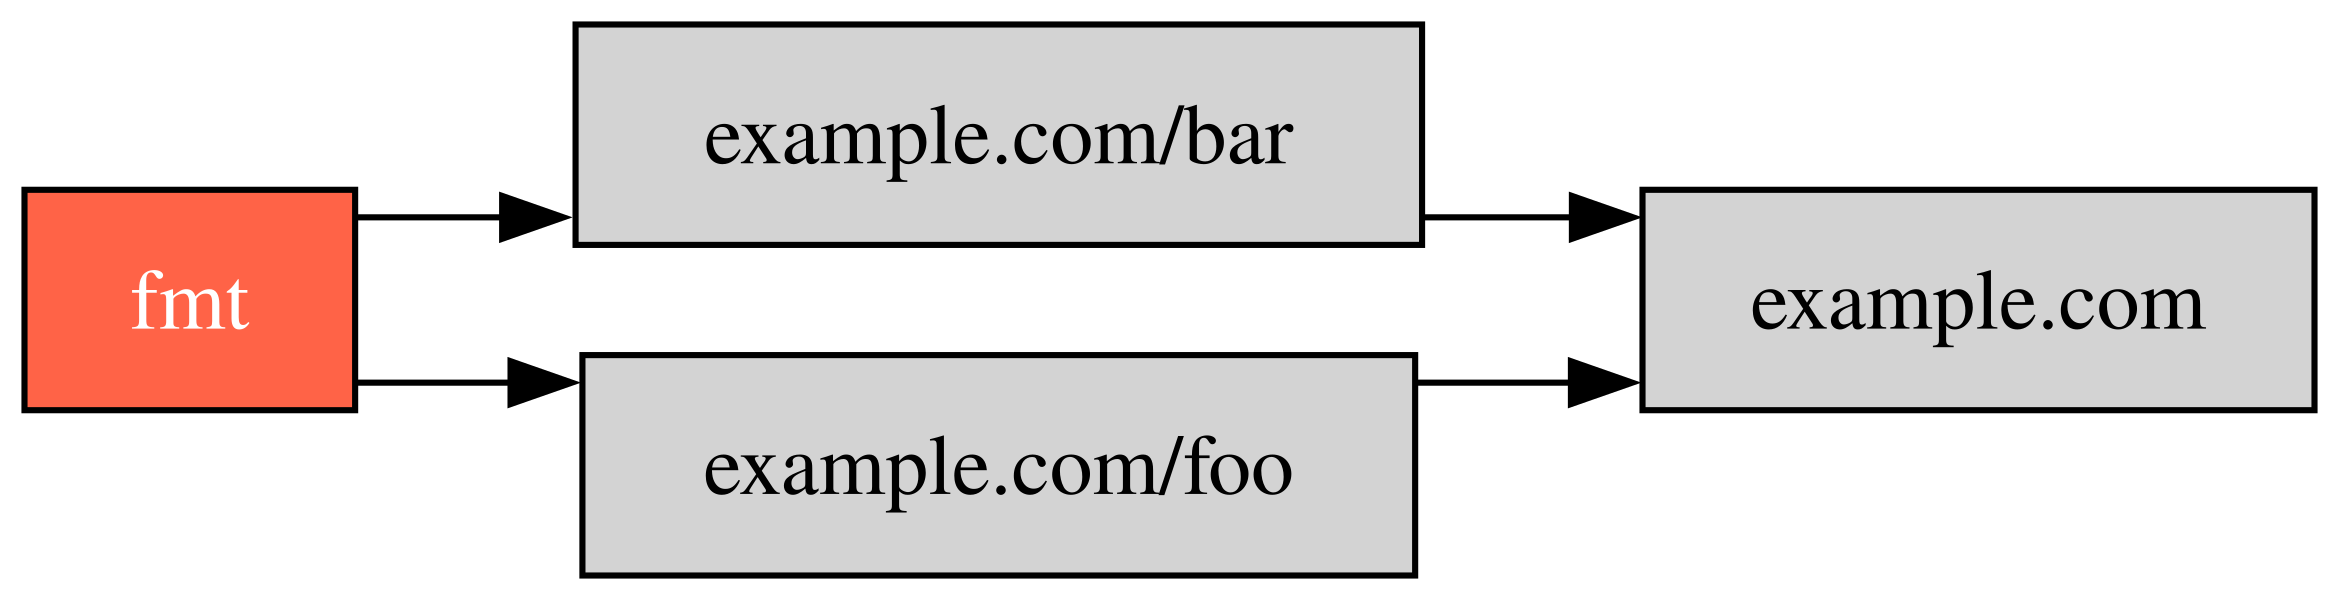
\includegraphics[width=.75\textwidth]{examples/example.com.png}
\caption{Visualização do grafo de um projeto simples, com dependências lineares.}
\label{fig:grafoExemplo}
\end{figure}

\FloatBarrier

\subsubsection{Caso 2: Biblioteca de CLI (Cobra)}
A Figura \ref{fig:exemplo-2} exibe o grafo de dependências da popular biblioteca `Cobra`, usada para criar aplicações de linha de comando (CLI). A estrutura aqui é mais complexa. Observamos um nó central (`github.com/spf13/cobra`) do qual muitos outros pacotes dependem. Também vemos dependências de pacotes externos como `github.com/spf13/pflag`, que gerencia flags de comando. Este tipo de grafo, com um "hub" central, é típico de bibliotecas de framework, onde um pacote principal oferece a funcionalidade central que é estendida por outros.

\begin{figure}[htbp]
\centering
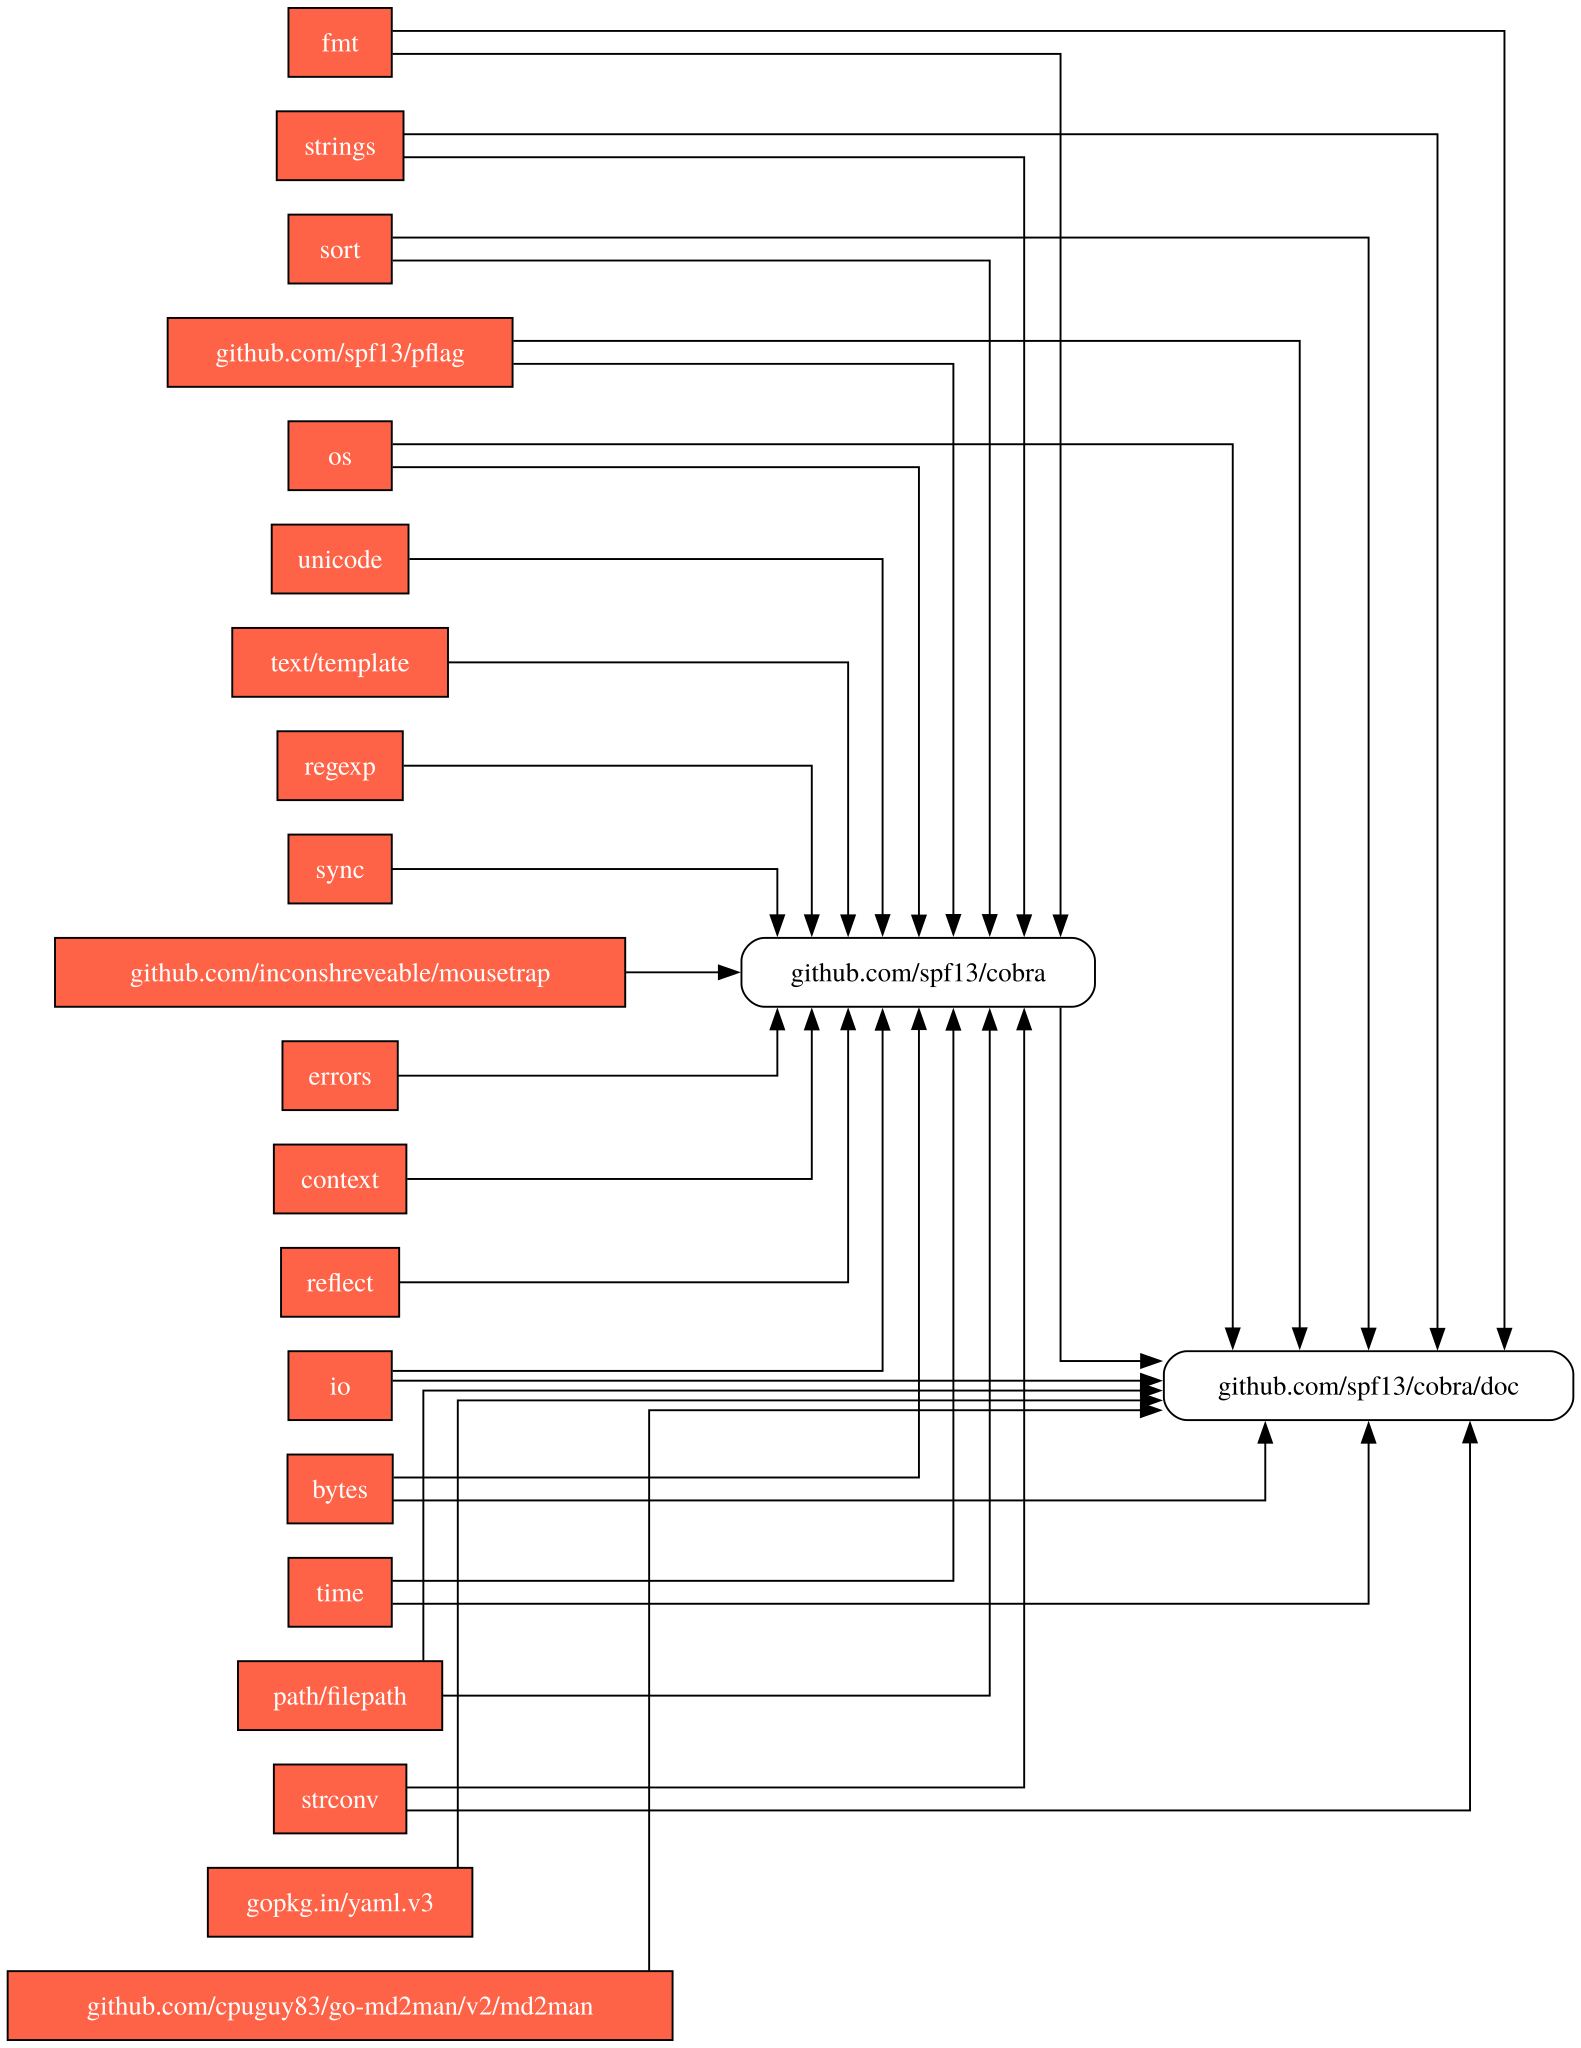
\includegraphics[width=.6\textwidth]{examples/github.com_spf13_cobra.png}
\caption{Grafo de dependências da biblioteca `Cobra`, mostrando uma estrutura de hub central.}
\label{fig:exemplo-2}
\end{figure}

\FloatBarrier

\subsubsection{Caso 3: Biblioteca de Utilitários (Posener/CMD)}
A Figura \ref{fig:exemplo-3} mostra o grafo da biblioteca `github.com/posener/cmd`. Este grafo exibe uma estrutura diferente, mais "larga" e menos profunda que as anteriores. Isso sugere que a biblioteca é uma coleção de utilitários mais ou menos independentes, que compartilham algumas dependências comuns (como o pacote `context`), mas não formam uma hierarquia rígida. A ferramenta revela que a arquitetura é altamente modular e de baixo acoplamento entre seus diferentes componentes.

\begin{figure}[htbp]
\centering
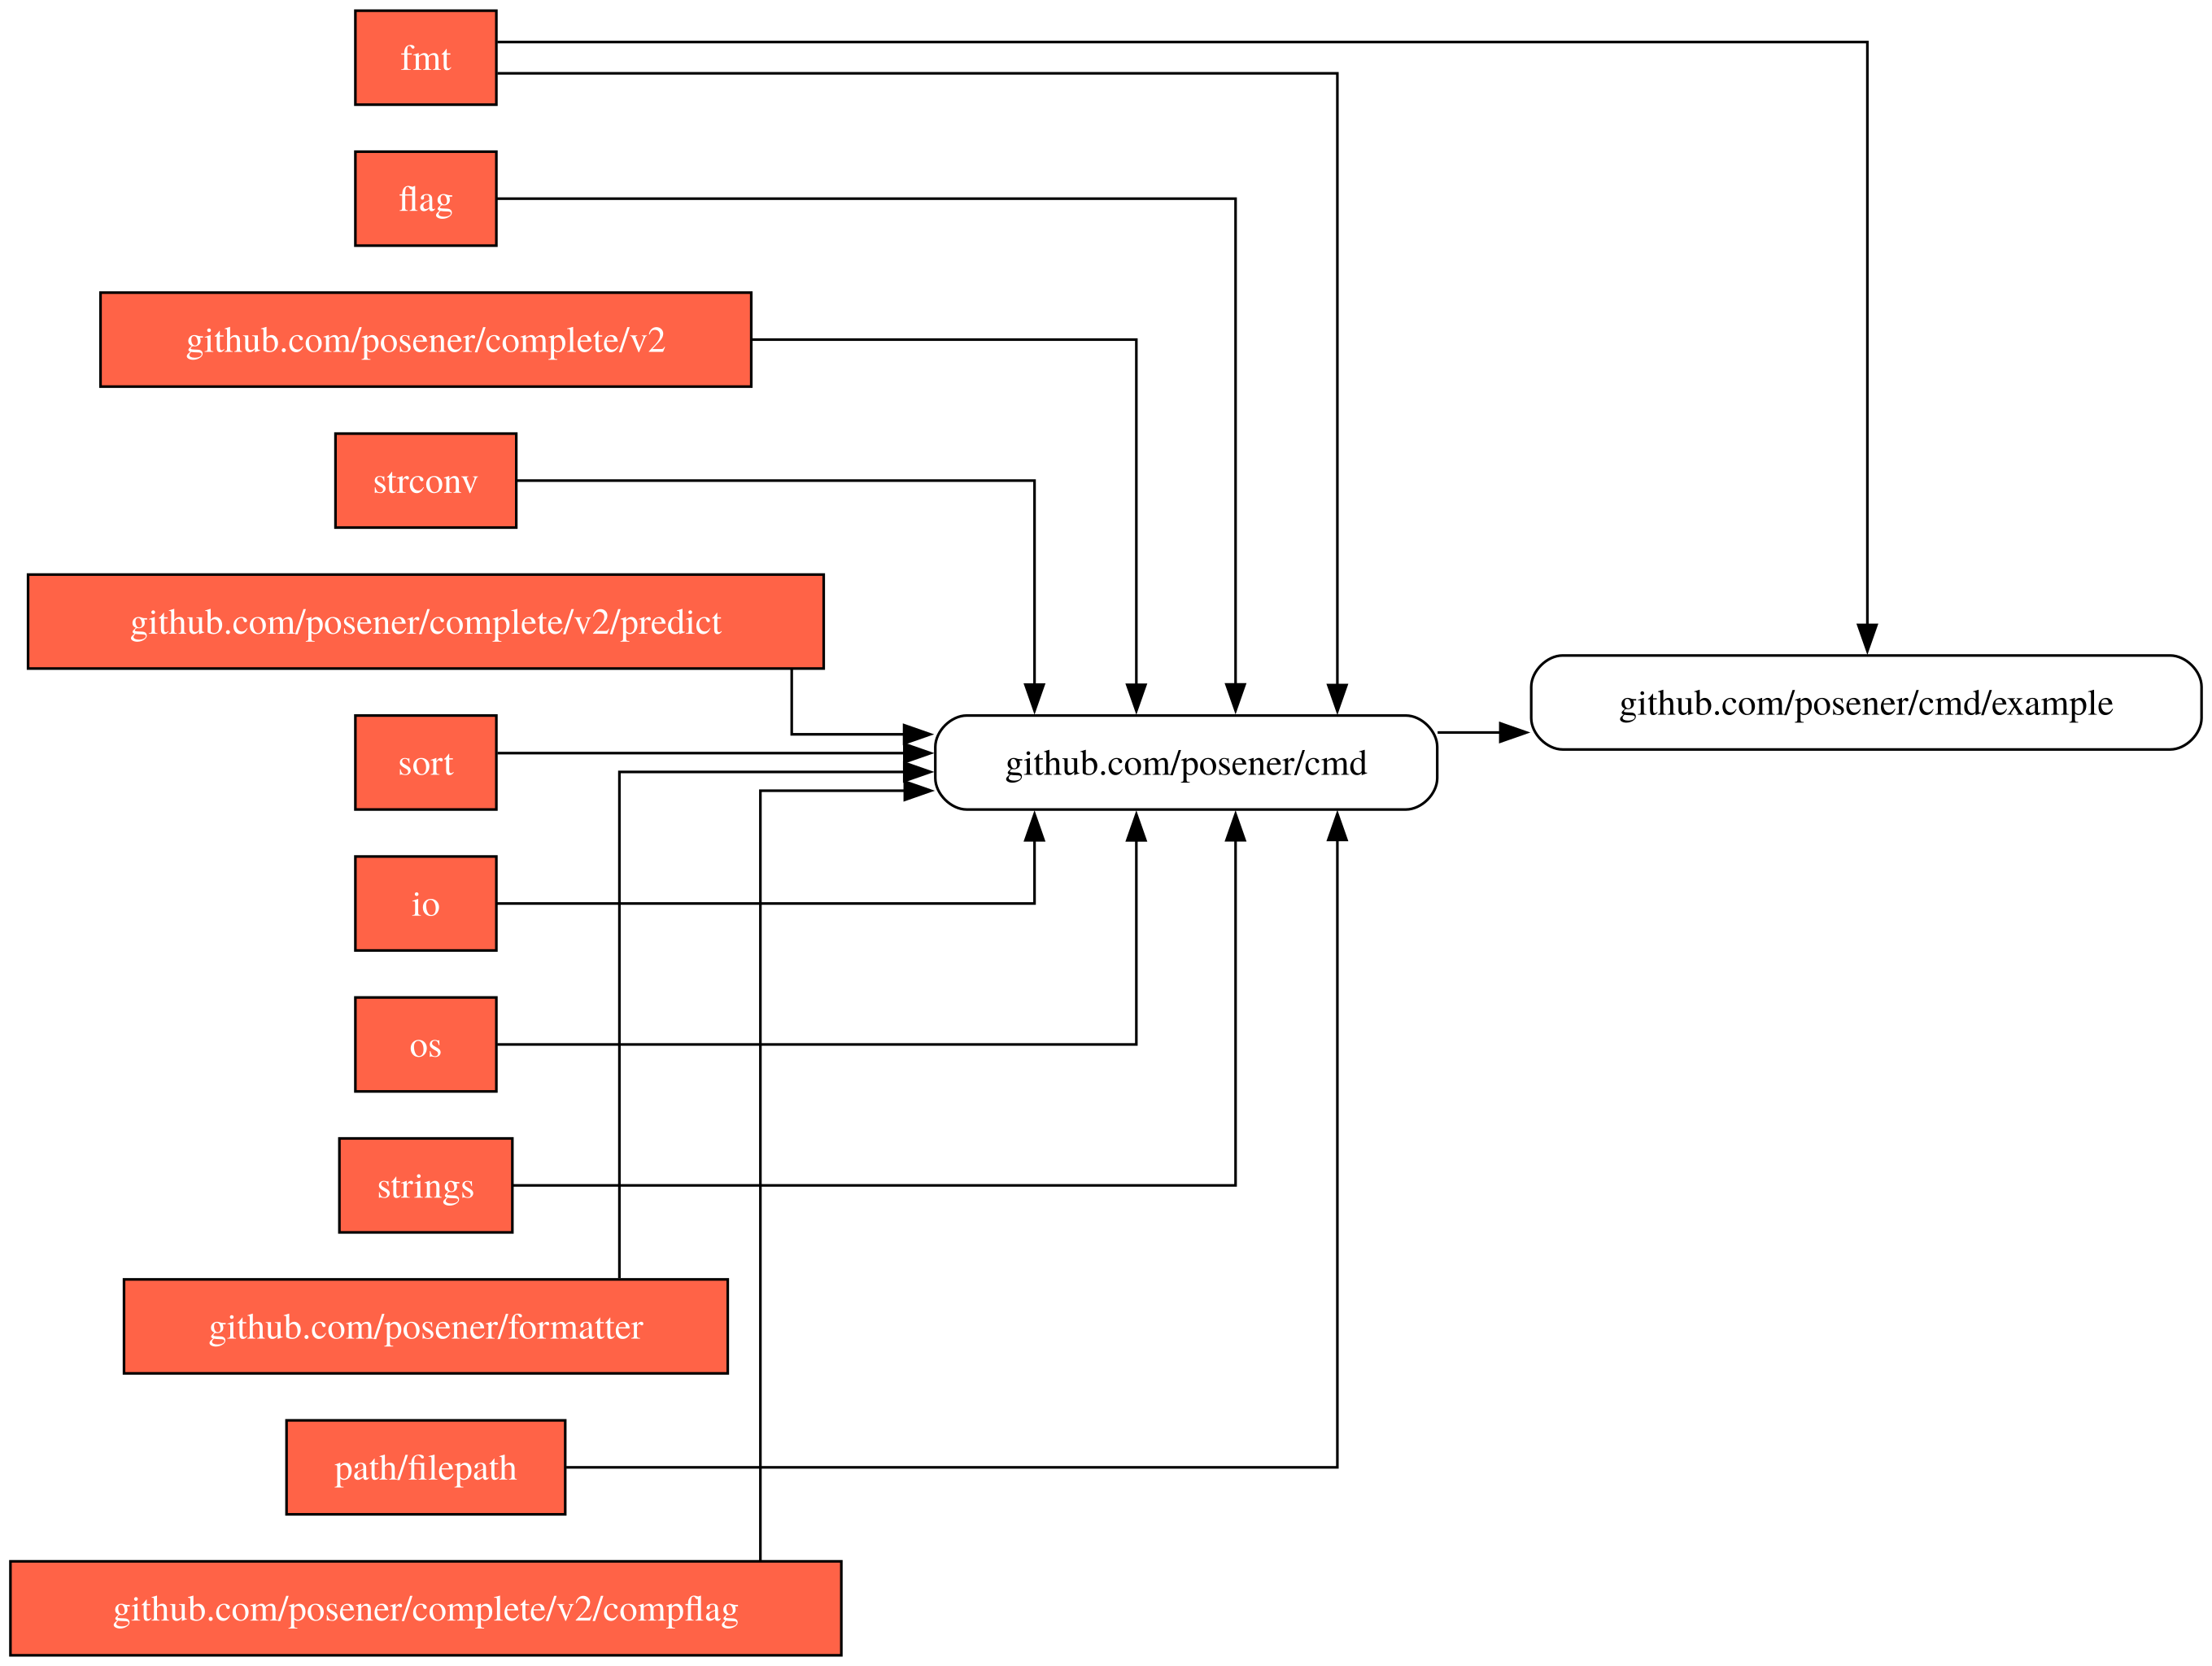
\includegraphics[width=.6\textwidth]{examples/github.com_posener_cmd.png}
\caption{Grafo de dependências da biblioteca `posener/cmd`, exibindo uma arquitetura modular e de baixo acoplamento.}
\label{fig:exemplo-3}
\end{figure}

\FloatBarrier

\subsection{Discussão dos Resultados}
A análise dos três casos demonstra a utilidade da ferramenta para diferentes tipos de projeto. Para aplicações simples, ela valida a arquitetura. Para bibliotecas complexas, ela revela padrões de design, como hubs centrais ou arquiteturas modulares. A capacidade de diferenciar visualmente pacotes internos e externos (coloridos de forma distinta) e de alinhar os pacotes por camada de dependência oferece uma visão imediata sobre a estrutura e a ordem de compilação, facilitando a depuração e o onboarding de novos desenvolvedores.

\section{Conclusão}
Este trabalho apresentou uma solução computacional para o problema de gestão de dependências em projetos Go. A modelagem do sistema de pacotes como um grafo direcionado provou-se eficaz, e a aplicação da ordenação topológica através do algoritmo de Kahn \cite{kahn1962} permitiu determinar a sequência de compilação segura e estruturar a visualização dos resultados de forma intuitiva. A ferramenta cumpre com sucesso os requisitos propostos, analisando o código-fonte, construindo um modelo em grafo e apresentando os resultados de forma clara. A capacidade de detectar ciclos de dependência é um recurso valioso para evitar erros comuns em projetos de grande porte.

\subsection{Trabalhos Futuros}
Apesar de funcional, a ferramenta pode ser estendida. Como trabalhos futuros, sugere-se:
\begin{itemize}
    \item \textbf{Análise de Desempenho:} Testar a ferramenta em repositórios extremamente grandes (e.g., Kubernetes).
    \item \textbf{Parser Avançado:} Substituir as expressões regulares por um parser de AST, tornando a extração de importações mais robusta.
    \item \textbf{Integração com IDEs:} Desenvolver um plugin para editores como o VS Code para exibir o grafo em tempo real.
    \item \textbf{Análise de "Peso" das Arestas:} Estender o modelo para incluir métricas de acoplamento.
\end{itemize}

\bibliographystyle{sbc}
\bibliography{sbc-template.bib}

\end{document}
